% Created 2023-04-13 Thu 23:20
% Intended LaTeX compiler: xelatex
\documentclass[manuscript,screen,review]{acmart}


\bibliographystyle{ACM-Reference-Format}
\author{30093813}
\date{\today}
\title{NLP Project Report: Corpus-Specific Automatic Hyperlinking}
\hypersetup{
 pdfauthor={30093813},
 pdftitle={NLP Project Report: Corpus-Specific Automatic Hyperlinking},
 pdfkeywords={},
 pdfsubject={},
 pdfcreator={Emacs 28.2 (Org mode 9.5.5)},
 pdflang={English}}
\usepackage{natbib}
\begin{document}

\maketitle

\section*{Introduction}
\label{sec:org4f12b5b}

\subsection*{Problem definition}
\label{sec:org8d466f4}
This project will attempt to address the problems resulting from the
necessity for manual linking in educational material. In particular,
educational material often requires large amounts of repetitive
linking to related explanatory material as it uses domain-specific
terminology. This results in at least one of two sets of problems:

\begin{enumerate}
\item The authors of the educational material under-link, meaning they
use domain-specific terminology without linking to its
corresponding explanatory material, resulting in decreased
effectiveness of the educational material as its consumers now face
a higher barrier-to-entry.
\item The authors of the educational material manually link, resulting in
decreased efficiency during authoring, a higher chance of error in
linking, and an increased cost of maintenance as the educational
material evolves and links change.
\end{enumerate}


An example corpus of educational material which suffers from these
problems is the \texttt{scikit-learn} \citep{scikit-learn} \href{https://scikit-learn.org/stable/index.html}{documentation}. The
documentation contains a wealth of knowledge relating not only to the
library itself but machine learning as a whole, however for a reader
who is new to the domains of machine learning and statistics it can be
quite opaque as it consistently uses domain specific terminology. For
example, the first sentence in the user guide reads:

\begin{quote}
``The following are a set of methods intended for regression in which
the target value is expected to be a linear combination of the
features.''
\end{quote}

There isn't anything inherently wrong with this as the documentation
assumes working knowledge of the domain, however it has potential for
improvement. For example, the glossary already contains definitions
for the terms ``target'' \citep{scikit-learn-gloss-term-Y} and ``feature''
\citep{scikit-learn-gloss-term-feature}, and even has an example of
``feature'' being used and linked in context
\citep{scikit-learn-gloss-term-X}. However a reader who is new to the
domain who stumbles across such articles will likely be confused, and
educational material would ideally provide an obvious path for
resolving that confusion.

\subsection*{Approach}
\label{sec:orgd904059}
This project attempts to address the root of the problem: it is easier
to not link than to link. The project explores the NLP techniques that
can be used to enable the automatic identification of the spans of a
document which should be linked, and the pairing of such spans with
their appropriate links.

The project uses the \texttt{scikit-learn} \citep{scikit-learn} documentation
as a dataset. It parses the links from the HTML using Pandoc
\citep{pandoc-homepage}, processes the data using Python, and trains a
span classification pipeline using SpaCy \citep{spacy}.

The project is in essence a supervised classification task, and as
such it will be evaluated using classification metrics such as those
listed in the \texttt{scikit-learn} user guide
\citep{scikit-learn-user-guide-classification-metrics}.

\subsection*{Related Work}
\label{sec:org93e8327}
This project falls under the category of text based entity linking
\citep{wikipedia-entity-linking}. More specifically, it is essentially
a system to support corpus-specific ``wikification'' of any corpus with
parse-able links (as opposed to being limited to linking to
Wikipedia). Existing approaches to text based entity linking typically
follow a two step process of first identifying entities
(a.k.a. keyword extraction) then matching them to their links (a.k.a
word sense disambiguation), and focus on using Wikipedia data
\citep{cucerzan-2007-large,wikify-mihalcea,wikigum}. Existing
approaches also make use of the additional metadata provided by
Wikipedia datasets, such as the entity categories and classes, to help
with the common problem of disambiguation. Existing approaches also
make heavy use of the existing links within the corpus to extract the
context and ``surface forms'' (different terms for the same entity) of
the entities. The most difficult problem appears to be that of
disambiguation. \citeauthor{entity-linking-bert} seems to represent
the state-of-the-art in entity linking and uses the newer technique of
transformer models with BERT to learn the context of the entities in a
document. With SpaCy's recent support for training transformer models
in pipelines, I explore a similar approach in this project.


\section*{Materials and Methods}
\label{sec:org52707f0}

\subsection*{Dataset and Link Extraction}
\label{sec:org083e034}
The dataset chosen was the \texttt{scikit-learn} documentation (GitHub source:
\url{https://github.com/scikit-learn/scikit-learn/tree/main/doc}, commit
\texttt{449940985c903f77678c0627cbc7a6267c3a54f9}). To extract the link data
from the documents, I wrote a tool which uses Pandoc
\citep{pandoc-homepage} to assign UUIDs to each link in each document,
wrap the link content with a special marker for later extraction,
store the UUID-to-link mapping in a JSON file, and convert the HTML to
plain text. Pandoc was chosen to make it easier to use the tool on
different datasets with different documentation formats. The tool also
has the option to narrow the link extraction to a particular element
within the HTML; this was used to only extract the main content of the
pages, while excluding the other HTML like the navigation bar. This
had the effect of greatly increasing link balance and relevance, as
the navigation elements were present on the majority of pages, and
they contained the same links on every page.

\subsection*{Link Normalization}
\label{sec:org84748c5}

After the link data and raw text is extracted, Python is used for
further processing of the links. The dataset consists of 996 documents
with a total length of 1100122 words (according to the \texttt{wc} command line
utility). Unprocessed, the dataset consists of a total of 16905 unique
links. Multiple processing steps were used to account for different
link forms: the links were lowercased, ``http'' forms of existing
``https'' links were converted to ``https'', Python's \texttt{urllib} was used for
normalization, and relative links were normalized. Following this
processing, the dataset consisted of 16162 unique links.

\subsection*{Link Occurrence Filtering}
\label{sec:org279658e}

Links occurrences were further filtered by removing cases where the
occurrence's user readable text did not contain at least 3
alphanumeric characters. This was implemented to prevent the model
from trying to learn from uninformative text which does not have any
special relation to the particular link it corresponds to. For
example, the corpus contains many occurrences of ``¶'', which is used
generally to link to headers, so that same span is associated with
many different links. Furthermore, these non-alphanumeric spans are most
likely generated text as opposed to user authored text, so there isn't
any need to automatically link these spans.

Following this filtering, the dataset contained 9715 unique links.

\subsection*{Generating Training Examples}
\label{sec:orge1c2da2}

The dataset has the property that the majority of the text is a
negative sample (it does not contain any links). To deal with this,
training examples were generated as follows:

\begin{enumerate}
\item A sliding window with a width of three sentences was run over each
document. If the window contains any link spans, that window is
added as a training example. Sentences were predicted by SpaCy's
\href{https://spacy.io/usage/linguistic-features\#sbd-component}{Sentencizer}. Other sentence splitting strategies provided by SpaCy
don't seem to work as well, likely due to the unique formatting of
the corpus (for example it includes code blocks).
\item Cases where the links cross sentence boundaries and are not
included in a training example are given a context of 10 words on
either side, and this is included as a training example.
\end{enumerate}


This process results in 11315 training examples.

\subsection*{Reducing Class Count}
\label{sec:org1bfe0a8}

After the above pre-processing, the dataset still contains far too
many classes for classification.

The majority of links have very few occurrences; Figure \ref{fig:org691fd04}
illustrates the exponentially decreasing relationship between the
minimum occurrence count and the number of classes meeting that
minimum. Over 80\% of the links in the dataset have only one example,
and only 157 links have more than 10 examples. Table \ref{tab:org0e24505}
summarizes the number of classes for a few milestone thresholds.

\begin{figure}[htbp]
\centering
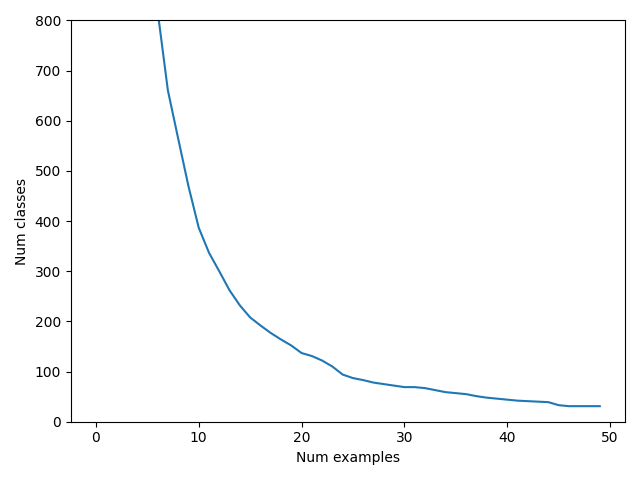
\includegraphics[width=.9\linewidth]{images/numclasses.png}
\caption{\label{fig:org691fd04}Distribution of minimum example count}
\end{figure}

\begin{table}[htbp]
\caption{\label{tab:org0e24505}Counts of classes for different thresholds}
\centering
\begin{tabular}{rr}
Minimum examples & Number of classes\\
\hline
5 & 453\\
10 & 157\\
15 & 89\\
20 & 49\\
25 & 30\\
30 & 23\\
\end{tabular}
\end{table}

To help reduce the number of classes, we can focus on the links with
many examples; fortunately this is suitable for the application,
because links with many examples are more likely to be used again. The
majority of experiments used a threshold of 15 as this threshold
provides a good balance between the number of training samples per
link and the number of classes to predict, making for a reasonable
task for the model. A threshold of 15 also allows for a reasonable
number of links, improving the model's overall utility.

\subsection*{Train/Test Splitting}
\label{sec:org713ba6f}

To split the data into training and testing sets, the main challenge
is in keeping the classes balanced, as a single training example can
contain multiple class counts. Originally I wrote a custom script to
search for a balanced split. This script also operated on entire
documents, making it harder to balance classes as the classes came in
large, fixed clusters. However, if we view the problem as a
multi-label classification problem for the purposes of splitting (even
though this is not accurate for the actual final task of the model),
we can utilize the pre-existing library scikit-multilearn
\citep{skmultilearn} to do the splitting. In particular, the library
provides an implementation of a multi-label stratification algorithm
\citep{multilabelstrat2,multilabelstrat1}. To utilize the algorithm,
one can one-hot encode the label space with a \(n \times m\) matrix, where
\(n\) is the number of training examples, and \(m\) is the number of
classes. This is not a perfect representation as a single training
example may contain multiple instances of the same link, however the
algorithm ends up working very well for the task, providing a balanced
split with each class containing roughly proportionate amounts in the
training and testing sets. A test size of 33\% is used for most
experiments.

Following the training and testing split, under-sampling is performed
to further balance the class counts, as some classes are far more
prevalent than others and we don't want the model to become biased
towards these links. I tried to use imbalanced-learn's
\citep{imbalanced-learn} \texttt{RandomUnderSampler}, however the library does
not support multi-label datasets, and while there are ways to work
around this, they ultimately don't provide a great balance of classes.

I found that manual under-sampling using the following algorithm
provides a good balance:

\begin{enumerate}
\item Keep a running count of the number of occurrences for each class,
and find the minimum number of occurrences for a class
\item For each document, count the number of occurrences of each class in
the document and remove the document if subtracting those
occurrences keeps all the classes above the minimum
\end{enumerate}


For this particular dataset, this algorithm provided a perfect balance
(although that may not be the case for other datasets). With a minimum
threshold of 15 and a test size of 33\%, all 89 classes in the training
set contained 10 examples each, and all classes in the testing set
contained 5 examples each, with both the training and testing sets
having the same sets of classes. The dataset then consists of 786
training samples and 406 testing samples, 55740 total words (5575
unique), with spans containing 1 to 3 tokens with distribution: 1
(45.98\%), 2 (27.23\%), 3 (26.79\%). The 10 most common span tokens are:
``.'', ``pipeline'', ``fit'', ``gridsearchcv'', ``linear\_model'', ``pca'',
``sgdclassifier'', ``ensemble'', ``sklearn.model\_selection'',
``sklearn.ensemble''.

\subsection*{Model Training}
\label{sec:org4c1a630}

SpaCy \citep{spacy} is used for building a classifier. All training
and testing data is stored in SpaCy's binary data format using \texttt{DocBin},
and SpaCy's built-in training process is used for all training. The
full model configuration can be found \href{https://github.com/rynoV/CPSC-599-NLP-project/blob/master/config.cfg}{on GitHub}. The pipeline consists
of SpaCy's default tokenizer followed by two components: a pre-trained
DistilBERT transformer \citep{distilbert} from the Hugging Face
\citep{hugging-face} library, followed by SpaCy's \texttt{SpanCategorizer}
component.

The DistilBERT transformer was chosen to allow for the use of span
context during classification, in the hopes of creating a more
sophisticated classification strategy. It is also well suited for this
application due to its reduced size, and its potential for speed
improvements on CPUs with techniques such as those described in
\citeauthor{fastdistilbert}. The span categorizer is set up to
categorize the spans generated during the data processing above, and
it is connected to the transformer. Both components are trained
together, with the span categorizer using the transformer's outputs as
features. All training was performed on unpaid Google Colab GPUs.

The full training command used is:

\begin{verbatim}
python -m spacy train config.cfg --output ./output --paths.train ./train.spacy --paths.dev ./test.spacy --gpu-id 0
\end{verbatim}

Minimal hyper-parameter tuning was performed due to time constraints
and because SpaCy's defaults provided good results. One difficulty
encountered was running out of GPU memory when training on the full
documents, and some tuning of batch sizes was required to reduce
memory usage. However after switching to smaller training examples,
the memory requirements were much smaller and no longer an issue.

\section*{Results}
\label{sec:org4c96a5c}
Multiple iterations of the model were trained as the data preparation
progressed. For the results, I will focus on the results of the model
with the final (and best) data preparation (described above). The
overall classification scores are shown below:

\begin{verbatim}
import json
with open('output/model-best9/meta.json') as f:
    data = json.load(f)['performance']
print('Precision:', data['spans_sc_p'])
print('Recall:   ', data['spans_sc_r'])
print('F1-score: ', data['spans_sc_f'])
\end{verbatim}

\begin{verbatim}
Precision: 0.8923766816
Recall:    0.8943820225
F1-score:  0.8933782267
\end{verbatim}


Next are the scores for each class.

\begin{verbatim}
import pandas as pd
import os
import re
data = pd.read_csv(os.path.join('output', 'model-best9', 'results.csv'), index_col=0)
mlen = 60
def trunc_link(link):
    prefix = '...' if len(link) > mlen else ''
    return prefix + re.sub('_', ' ', link)[-min(len(link), mlen):]
data.index = data.index.map(trunc_link)
\end{verbatim}

Many of the classes end up with perfect scores. The proportion of such
classes is given:

\begin{verbatim}
f'{100 * data[data["f"] == 1].shape[0] / data.shape[0]:.2f}%'
\end{verbatim}

\begin{verbatim}
44.94%
\end{verbatim}


Table \ref{tab:org065b7ad} contains the scores for the classes which did
not receive perfect scores. Note that the ``support'' column contains
the number of samples tested, and ``p'', ``r'', and ``f'' are precision,
recall, and F1-score, respectively.

\begin{verbatim}
df = data[(data['f'] != 1)]
df
\end{verbatim}

\begin{table}[htbp]
\caption{\label{tab:org065b7ad}Results without perfect F1-score}
\centering
\begin{tabular}{lrrrr}
 & p & r & f & support\\
\hline
glossary.html\#term-decision function & 0.5 & 0.2 & 0.285714 & 5\\
\url{https://twitter.com/ogrisel} & 0.5 & 0.4 & 0.444444 & 5\\
\ldots{}ction.gridsearchcv.html\#sklearn.model selection.gridsearchcv & 0.5 & 0.4 & 0.444444 & 5\\
\ldots{}ted/sklearn.pipeline.pipeline.html\#sklearn.pipeline.pipeline & 0.666667 & 0.4 & 0.5 & 5\\
\ldots{}ction.gridsearchcv.html\#sklearn.model selection.gridsearchcv & 0.428571 & 0.6 & 0.5 & 5\\
glossary.html\#term-predict & 1 & 0.4 & 0.571429 & 5\\
\#term-fit & 0.6 & 0.6 & 0.6 & 5\\
glossary.html\#term-predict proba & 0.6 & 0.6 & 0.6 & 5\\
\ldots{}ted/sklearn.decomposition.pca.html\#sklearn.decomposition.pca & 0.75 & 0.6 & 0.666667 & 5\\
glossary.html\#term-fit & 0.75 & 0.6 & 0.666667 & 5\\
\ldots{}ted/sklearn.decomposition.pca.html\#sklearn.decomposition.pca & 0.571429 & 0.8 & 0.666667 & 5\\
\ldots{}learn.linear model.ridgecv.html\#sklearn.linear model.ridgecv & 1 & 0.6 & 0.75 & 5\\
\ldots{}lectfrommodel.html\#sklearn.feature selection.selectfrommodel & 1 & 0.6 & 0.75 & 5\\
\url{https://sites.google.com/site/peterprettenhofer/} & 0.625 & 1 & 0.769231 & 5\\
\url{http://www.montefiore.ulg.ac.be/\~glouppe/} & 0.8 & 0.8 & 0.8 & 5\\
\ldots{}arn.pipeline.featureunion.html\#sklearn.pipeline.featureunion & 0.8 & 0.8 & 0.8 & 5\\
\ldots{}izedsearchcv.html\#sklearn.model selection.randomizedsearchcv & 0.8 & 0.8 & 0.8 & 5\\
\ldots{} model.sgdclassifier.html\#sklearn.linear model.sgdclassifier & 0.8 & 0.8 & 0.8 & 5\\
generated/sklearn.svm.linearsvc.html\#sklearn.svm.linearsvc & 0.714286 & 1 & 0.833333 & 5\\
\url{https://gael-varoquaux.info} & 0.714286 & 1 & 0.833333 & 5\\
\url{https://github.com/ogrisel} & 0.714286 & 1 & 0.833333 & 5\\
\ldots{}ose.columntransformer.html\#sklearn.compose.columntransformer & 1 & 0.8 & 0.888889 & 5\\
\url{https://github.com/thomasjpfan} & 1 & 0.8 & 0.888889 & 5\\
\url{http://www.mblondel.org} & 1 & 0.8 & 0.888889 & 5\\
\ldots{}learn.impute.simpleimputer.html\#sklearn.impute.simpleimputer & 1 & 0.8 & 0.888889 & 5\\
\ldots{}n.naive bayes.gaussiannb.html\#sklearn.naive bayes.gaussiannb & 1 & 0.8 & 0.888889 & 5\\
classes.html\#module-sklearn.metrics.pairwise & 1 & 0.8 & 0.888889 & 5\\
\url{https://github.com/micky774} & 1 & 0.8 & 0.888889 & 5\\
\ldots{}gclassifier.html\#sklearn.ensemble.gradientboostingclassifier & 1 & 0.8 & 0.888889 & 5\\
\ldots{}.featurehasher.html\#sklearn.feature extraction.featurehasher & 1 & 0.8 & 0.888889 & 5\\
\ldots{}orestclassifier.html\#sklearn.ensemble.randomforestclassifier & 1 & 0.8 & 0.888889 & 5\\
\ldots{}tml\#sklearn.discriminant analysis.lineardiscriminantanalysis & 1 & 0.8 & 0.888889 & 5\\
\ldots{}impute.iterativeimputer.html\#sklearn.impute.iterativeimputer & 1 & 0.8 & 0.888889 & 5\\
\url{https://amueller.github.io/} & 0.833333 & 1 & 0.909091 & 5\\
\ldots{}ted/sklearn.pipeline.pipeline.html\#sklearn.pipeline.pipeline & 0.833333 & 1 & 0.909091 & 5\\
\url{https://github.com/qinhanmin2014} & 0.833333 & 1 & 0.909091 & 5\\
\ldots{} model.sgdclassifier.html\#sklearn.linear model.sgdclassifier & 0.833333 & 1 & 0.909091 & 5\\
\url{http://alexandre.gramfort.net} & 0.833333 & 1 & 0.909091 & 5\\
\ldots{}ssing.onehotencoder.html\#sklearn.preprocessing.onehotencoder & 0.833333 & 1 & 0.909091 & 5\\
\url{http://fa.bianp.net} & 0.833333 & 1 & 0.909091 & 5\\
\ldots{}localoutlierfactor.html\#sklearn.neighbors.localoutlierfactor & 0.833333 & 1 & 0.909091 & 5\\
\ldots{}essor.html\#sklearn.gaussian process.gaussianprocessregressor & 0.833333 & 1 & 0.909091 & 5\\
\url{https://github.com/larsmans} & 0.833333 & 1 & 0.909091 & 5\\
\ldots{}stimator.html\#sklearn.utils.estimator checks.check estimator & 0.833333 & 1 & 0.909091 & 5\\
generated/sklearn.svm.svr.html\#sklearn.svm.svr & 0.833333 & 1 & 0.909091 & 5\\
\ldots{}nerated/sklearn.svm.oneclasssvm.html\#sklearn.svm.oneclasssvm & 0.833333 & 1 & 0.909091 & 5\\
\ldots{}isticregression.html\#sklearn.linear model.logisticregression & 0.833333 & 1 & 0.909091 & 5\\
\url{https://github.com/lorentzenchr} & 0.833333 & 1 & 0.909091 & 5\\
\ldots{}letransformer.html\#sklearn.preprocessing.quantiletransformer & 0.833333 & 1 & 0.909091 & 5\\
\end{tabular}
\end{table}

As an example of the model's results, we can use SpaCy's Displacy tool
to render some predictions for the link ``glossary.html\#term-fit''. In
the following images, ``Reference'' shows a sample from the testing set
with its links bolded, and ``Predicted'' shows the model's predictions
bolded. Figure \ref{fig:org1eb226d} shows a case containing multiple
unique links and multiple occurrences of the same link, and the model
fails to identify any links. Figure \ref{fig:org8928d03} shows another
test case where the model made a prediction for the same span of text
as the reference.

\begin{figure}[htbp]
\centering
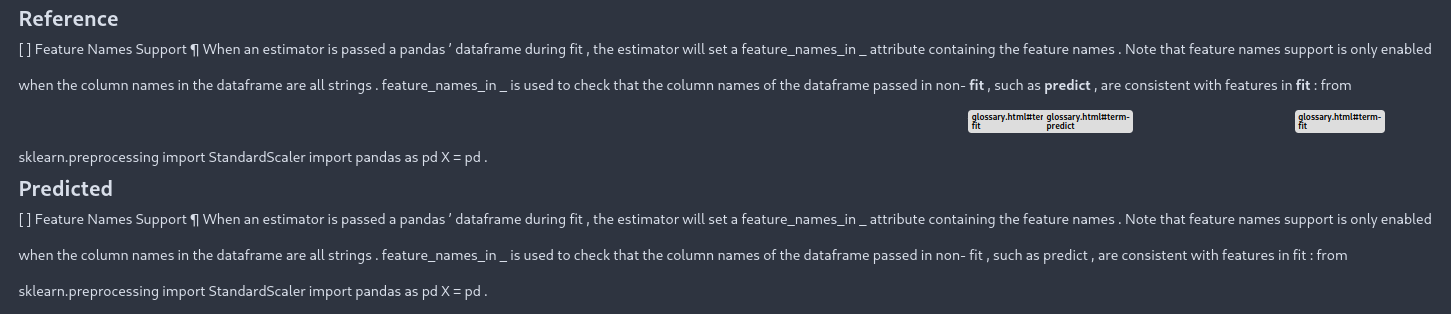
\includegraphics[width=450px]{screenshots/Writeup/2023-04-10_12-45-39_screenshot.png}
\caption{\label{fig:org1eb226d}An example from the testing set and the model's (lack of) predictions}
\end{figure}

\begin{figure}[htbp]
\centering
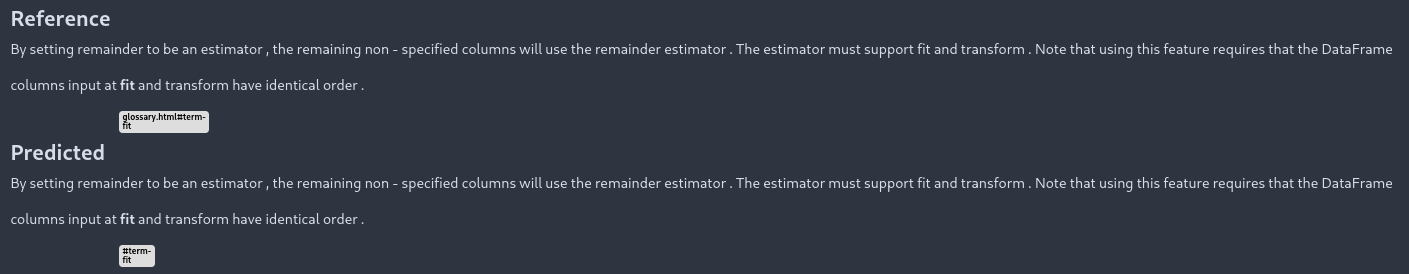
\includegraphics[width=450px]{screenshots/Writeup/2023-04-10_12-51-26_screenshot.png}
\caption{\label{fig:org8928d03}Another example from the testing set and the model's prediction}
\end{figure}

\section*{Discussion and Conclusion}
\label{sec:orgabd4620}

The results indicate that the system has some potential, however there
are some biases in the dataset that need to be considered when
evaluating the overall utility of the model. In particular, the
dataset is unbalanced with far more examples of links for unique
names, such as contributor names or function and class names, as
opposed to terms such as ``target'' and ``fit''. This is due largely to
the inclusion of all pages of the documentation in the dataset,
including changelogs (where contributors are frequently mentioned) and
API documentation (where function and class names are frequently
linked). It is also more common for function and class names to be
linked in the documentation than terms. Furthermore, the dataset
included repetitive automatically generated text, which is essentially
many instances of a template filled in with particular values. This
has the effect of the model learning very specific contexts for links
appearing in these templated texts. These biases in the dataset
account for many of the instances where the model achieved perfect
scores. In future iterations of the system, it would certainly be
preferable to include an option to filter automatically generated
text, as this not only biases the model but also makes the model learn
things that will likely not be used, as the text is automatically
generated and the system is for manually written text. A more
sophisticated duplicate detection algorithm could also catch these
instances of templated text.

One thing to note regarding the classification scores is that they
aren't perfect, because the evaluation samples and the dataset in
general is imperfect: by nature, the dataset contains false negatives
(spans that could be linked but aren't). For example, there are cases
where the model failed to classify the expected span of text, however
it classified another equally viable span of text correctly in the
same test example, but this is counted as a total failure. This
presence of false negatives is a general obstacle to be overcome by
the system, and may be addressed by adjusting the weight given to
negative samples, or providing a means of manual annotation of the
dataset by the authors.

One example of the model's hyper-specialization is for linked names
appearing in the changelogs, which almost exclusively appear at the
end of a line preceded by the same structure of text. Figure
\ref{fig:org7fd03e7} shows some of the training examples for one
such class, and figure \ref{fig:orgfd674a1} shows some predictions
of the model on text that I wrote. This class had a perfect
F1-score. The model appears to have learned a very specific
representation requiring the name to appear at the end or at the start
of the text, with a preference for it to be preceded by particular
text (the words ``by'' and ``and''). However, some useful properties of
the model are demonstrated here, in particular the ability to identify
similar forms such as when a middle initial is included in the name,
or it is misspelled.

\begin{figure}[htbp]
\centering
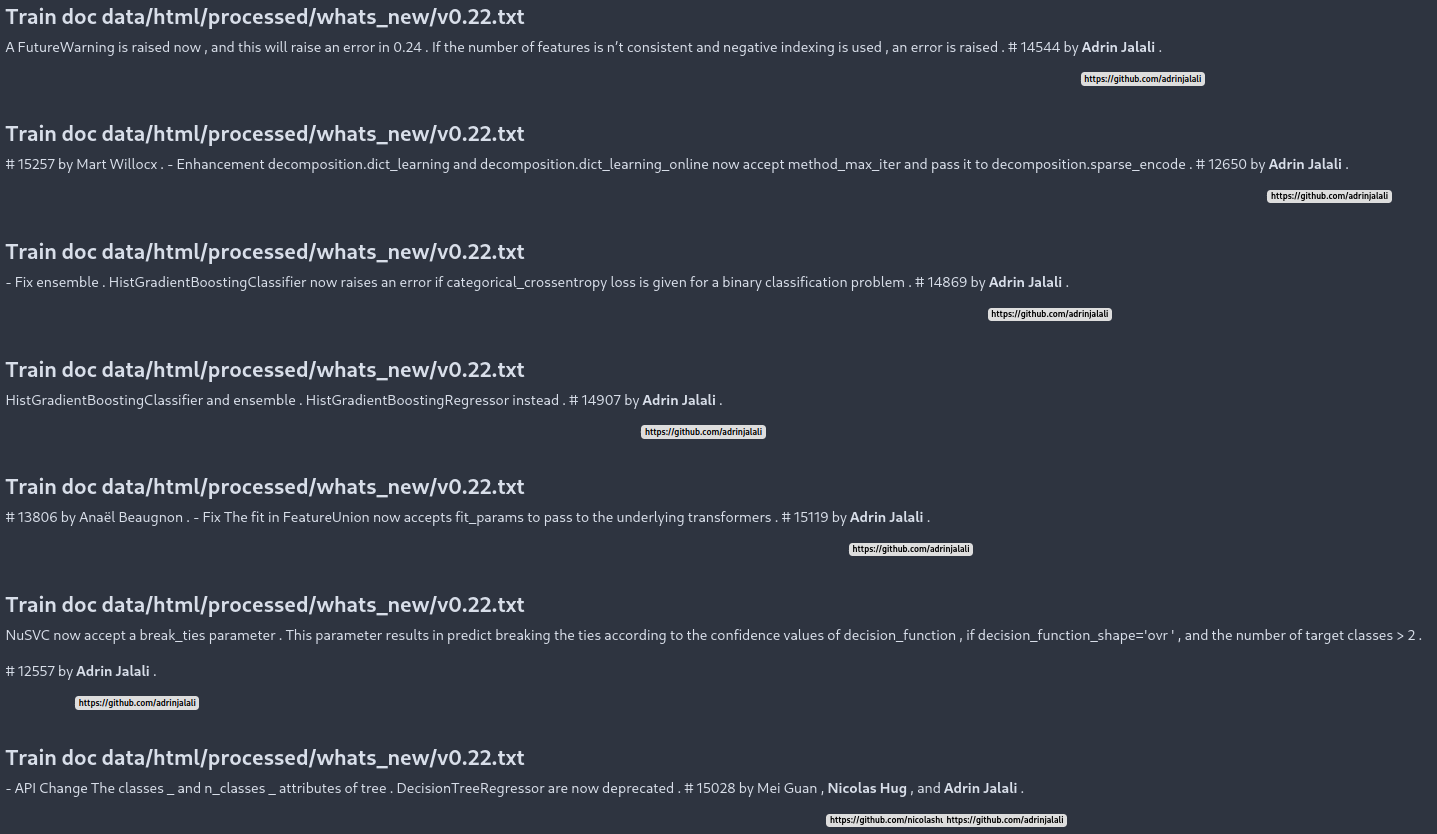
\includegraphics[width=450px]{screenshots/Writeup/2023-04-13_20-57-13_screenshot.png}
\caption{\label{fig:org7fd03e7}Training examples for the ``\url{https://github.com/adrinjalali}'' class}
\end{figure}

\begin{figure}[htbp]
\centering
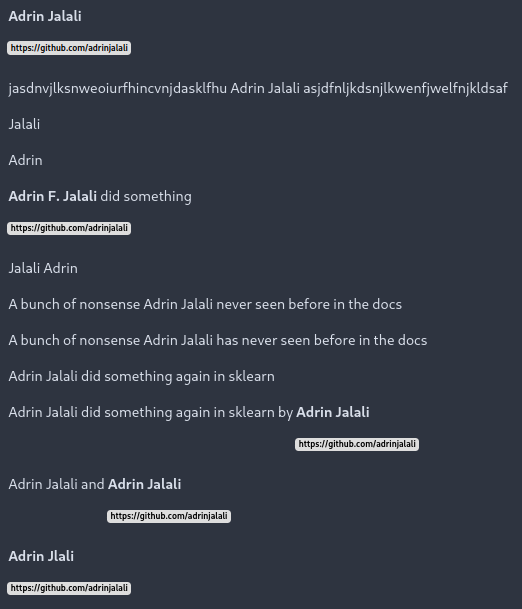
\includegraphics[width=200px]{screenshots/Writeup/2023-04-13_20-58-27_screenshot.png}
\caption{\label{fig:orgfd674a1}Predictions for the ``\url{https://github.com/adrinjalali}'' class}
\end{figure}

The ``\#term-fit'' class is an example of an imperfectly classified class
(0.6 F1-score) with a more diverse set of contexts where it
appears. Figure \ref{fig:orga486e08} shows a sample of the training
examples for this class, and \ref{fig:org07ffe02} again shows some
test cases. This example demonstrates the model's utilization of
context to learn more sophisticated representations for the
classes. In particular, we see that the model correctly does not
classify the usage of ``fit'' as a verb in the context of clothing as an
instance of this class. However we also see some potential
over-specialization, where the model seems to be requiring the word
``estimator'' to appear in some context before it will classify
``fit''. However this requirement is nuanced as demonstrated by the last
example, where the presence ``estimator'' is not sufficient to classify
``fit'' because the rest of the context doesn't match. It should also be
noted that this example is from an earlier version of the model, and
it is just being used to demonstrate the model's context learning
capabilities. In a later version of the model trained on more balanced
training data, it seems to have reduced this over-specialization.

\begin{figure}[htbp]
\centering
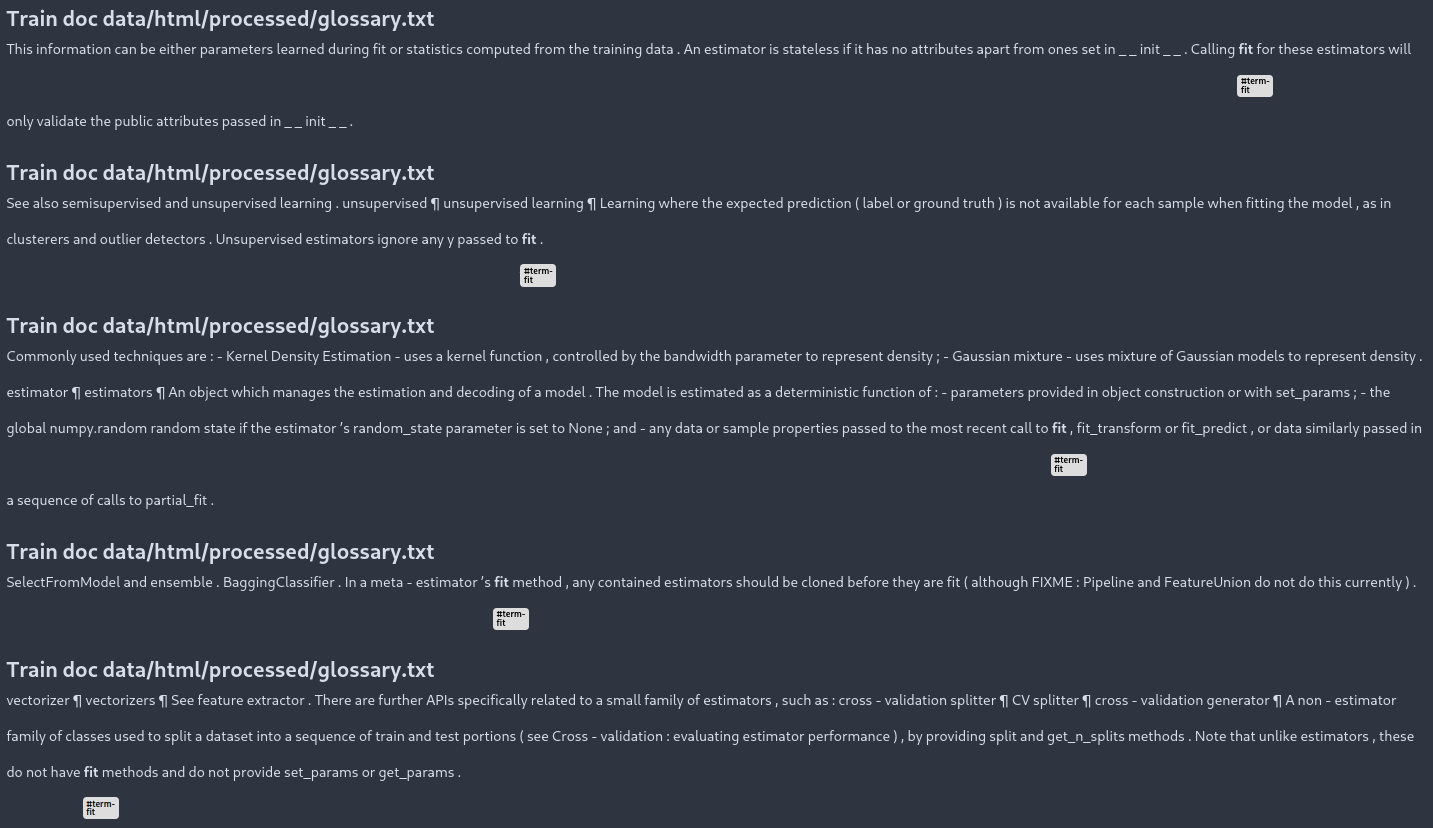
\includegraphics[width=450px]{screenshots/Writeup/2023-04-13_22-20-23_screenshot.png}
\caption{\label{fig:orga486e08}Training examples for the ``\#term-fit'' class}
\end{figure}

\begin{figure}[htbp]
\centering
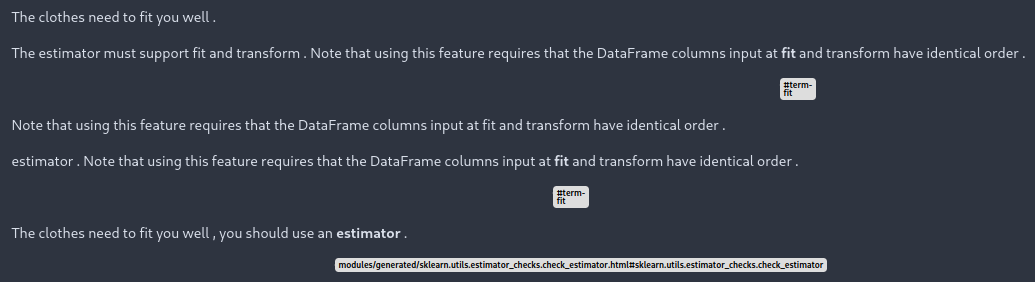
\includegraphics[width=450px]{screenshots/Writeup/2023-04-13_21-04-54_screenshot.png}
\caption{\label{fig:org07ffe02}Predictions for the ``\#term-fit'' class}
\end{figure}

In conclusion, the system demonstrates potential to become a
sophisticated and ``intelligent'' solution for corpus-tuned automatic
hyperlinking, however it requires more work to improve the system's
data processing to reduce bias in the data, and the system may require
some manual intervention by corpus authors to produce the best
results.

Future work would center around improving the system, likely focusing
on the following avenues:

\begin{itemize}
\item Handling false negatives: much of the text by nature contains false
negatives. If these false negatives get into the training data it
could give the model the wrong idea.
\begin{itemize}
\item One potential improvement may be to reduce the context around
examples, which would reduce the likelihood of false negatives
appearing in training
\item Could explore an approach like:
\url{https://github.com/doccano/spacy-partial-tagger}
\end{itemize}
\item Reducing bias in the data: data is very biased towards unique names
and biased against terms.
\begin{itemize}
\item This may just be a property of the dataset, in which case manual
annotation by the corpus authors would be required before the
system could improve
\item However this may be improved by providing document filter options,
for example to ignore things like API documentation, changelogs,
and generated text
\end{itemize}
\item Some potential data pre-processing improvements:
\begin{itemize}
\item Some equal links are not caught by normalization, in particular
links to a particular part of a page, from within the page and
without, for example ``\#pipeline'' and
``path/to/pipeline.html\#pipeline''. This could be handled by
incorporating the file path of the document in which the link
appears during normalization.
\item Try to increase diversity of training samples by prioritizing
unique span text during undersampling. The current undersampling
technique effectively chooses random samples, however an algorithm
which encourage more diversity may improve the system.
\item imbalanced-learn didn't work well for this task because it doesn't
support multi-label classification, however if some of the
imbalanced learning methods could be adapted to a multi-label
problem they may offer some improvement to the system.
\item Augmentation with something like \href{https://github.com/kennethenevoldsen/augmenty}{augmenty} \citep{augmenty} may
provide improvement.
\item One potential augmentation would be to vary the amount of context
in an example, to reduce the potential of the model leaning too
much on a particular amount of context.
\item Explore minimum alpha-numeric character requirement of 1 instead
of 3: the current pre-processing requires link text to have at
least 3 alpha-numeric characters, however some spans like ``X'' and
``Xt'' are being removed which may provide useful data.
\item The sentence sliding window technique could be improved by
ensuring the given span is in the middle of the set of
sentences. The current technique allows it to be in the end
sentences, making for inconsistent contexts in some cases.
\item More experimentation could be performed with the minimum class
occurrence threshold: a threshold of 15 was used for most
experiments, however a lower threshold may still allow for a
useful model while increasing the number of classes.
\end{itemize}
\item \url{https://spacy.io/universe/project/skweak} may be useful for
ensembling, for example combining the machine learning pipeline with
rule-based classifiers
\item A tool such as \url{https://spacy.io/universe/project/spacyfishing} can be
integrated into the system to facilitate pre-built wikipedia linking
on top of the corpus specific links
\end{itemize}

\bibliography{/home/calum/org/nlp}
\end{document}